\section{Introduction}\label{sec:intro}
An important question plaguing machine learning \cite{BenAli-1,Lecun,BenAli-2,Aliresponse,Mickens} is:
\begin{center}
\textbf{\emph{Is Deep Learning Alchemy?}}
\end{center}
The \emph{alchemy} question can further be broken down into sub-questions/issues/gaps as listed below. 

1. \emph{Training:} Despite a \emph{non-convex} loss surface, why is it possible for stochastic gradient descent (SGD) (and its variants) to achieve zero training error in standard deep neural networks (DNNs)?

2. \emph{Generalisation:} Standard DNNs are \emph{over-parameterised}, yet, when trained on data with true labels we observe good test performance. Does understanding deep learning require rethinking generalisation? \cite{ben}

3. \emph{Depth:} Approximation results show that more depth is better \cite{depth1,depth2}, i.e., deeper models can approximate more complicated target functions better than shallow models. Yet, when training on standard datasets, increasing the depth beyond a point adversely affects both training and test performance \cite{resnets}. This situation can be remedied by using \emph{skip connections} giving rise to residual neural networks. However, why increasing depth beyond a point hurts standard DNNs is still not understood satisfactorily. 

4. \emph{Depth vs Width:} Wider models \cite{wide1,wide2,wide3} have also been quite successful. While increasing either depth or width causes an increase in the number of model parameters, the trade-off between width and depth is not clearly understood.

5. \emph{Functionality:} The roles of the basic parts namely weights and activation have not been clearly understood.

6. \emph{Uninterpretablity of Learnt Representation:} The commonly held view of feature learning is that lower level features are learnt in the initial layers and as one proceeds in depth more sophisticated features are learnt in the higher levels and the final layer learns a linear model in the features given by the output of the penultimate layer. However, there is no straightforward way to interpret the features learnt in the hidden layers.

7. There is a gap between \emph{universal approximation results} which characterise the class of functions representable by DNNs and \emph{practical} DNNs that are trained using SGD (and variants) starting from randomly initialised weights. Further, the performance of DNNs are evaluated on standard datasets such as MNIST and CIFAR-10. 

\subsection{Related Work}
\FloatBarrier
\begin{figure}[h]
\resizebox{\columnwidth}{!}{
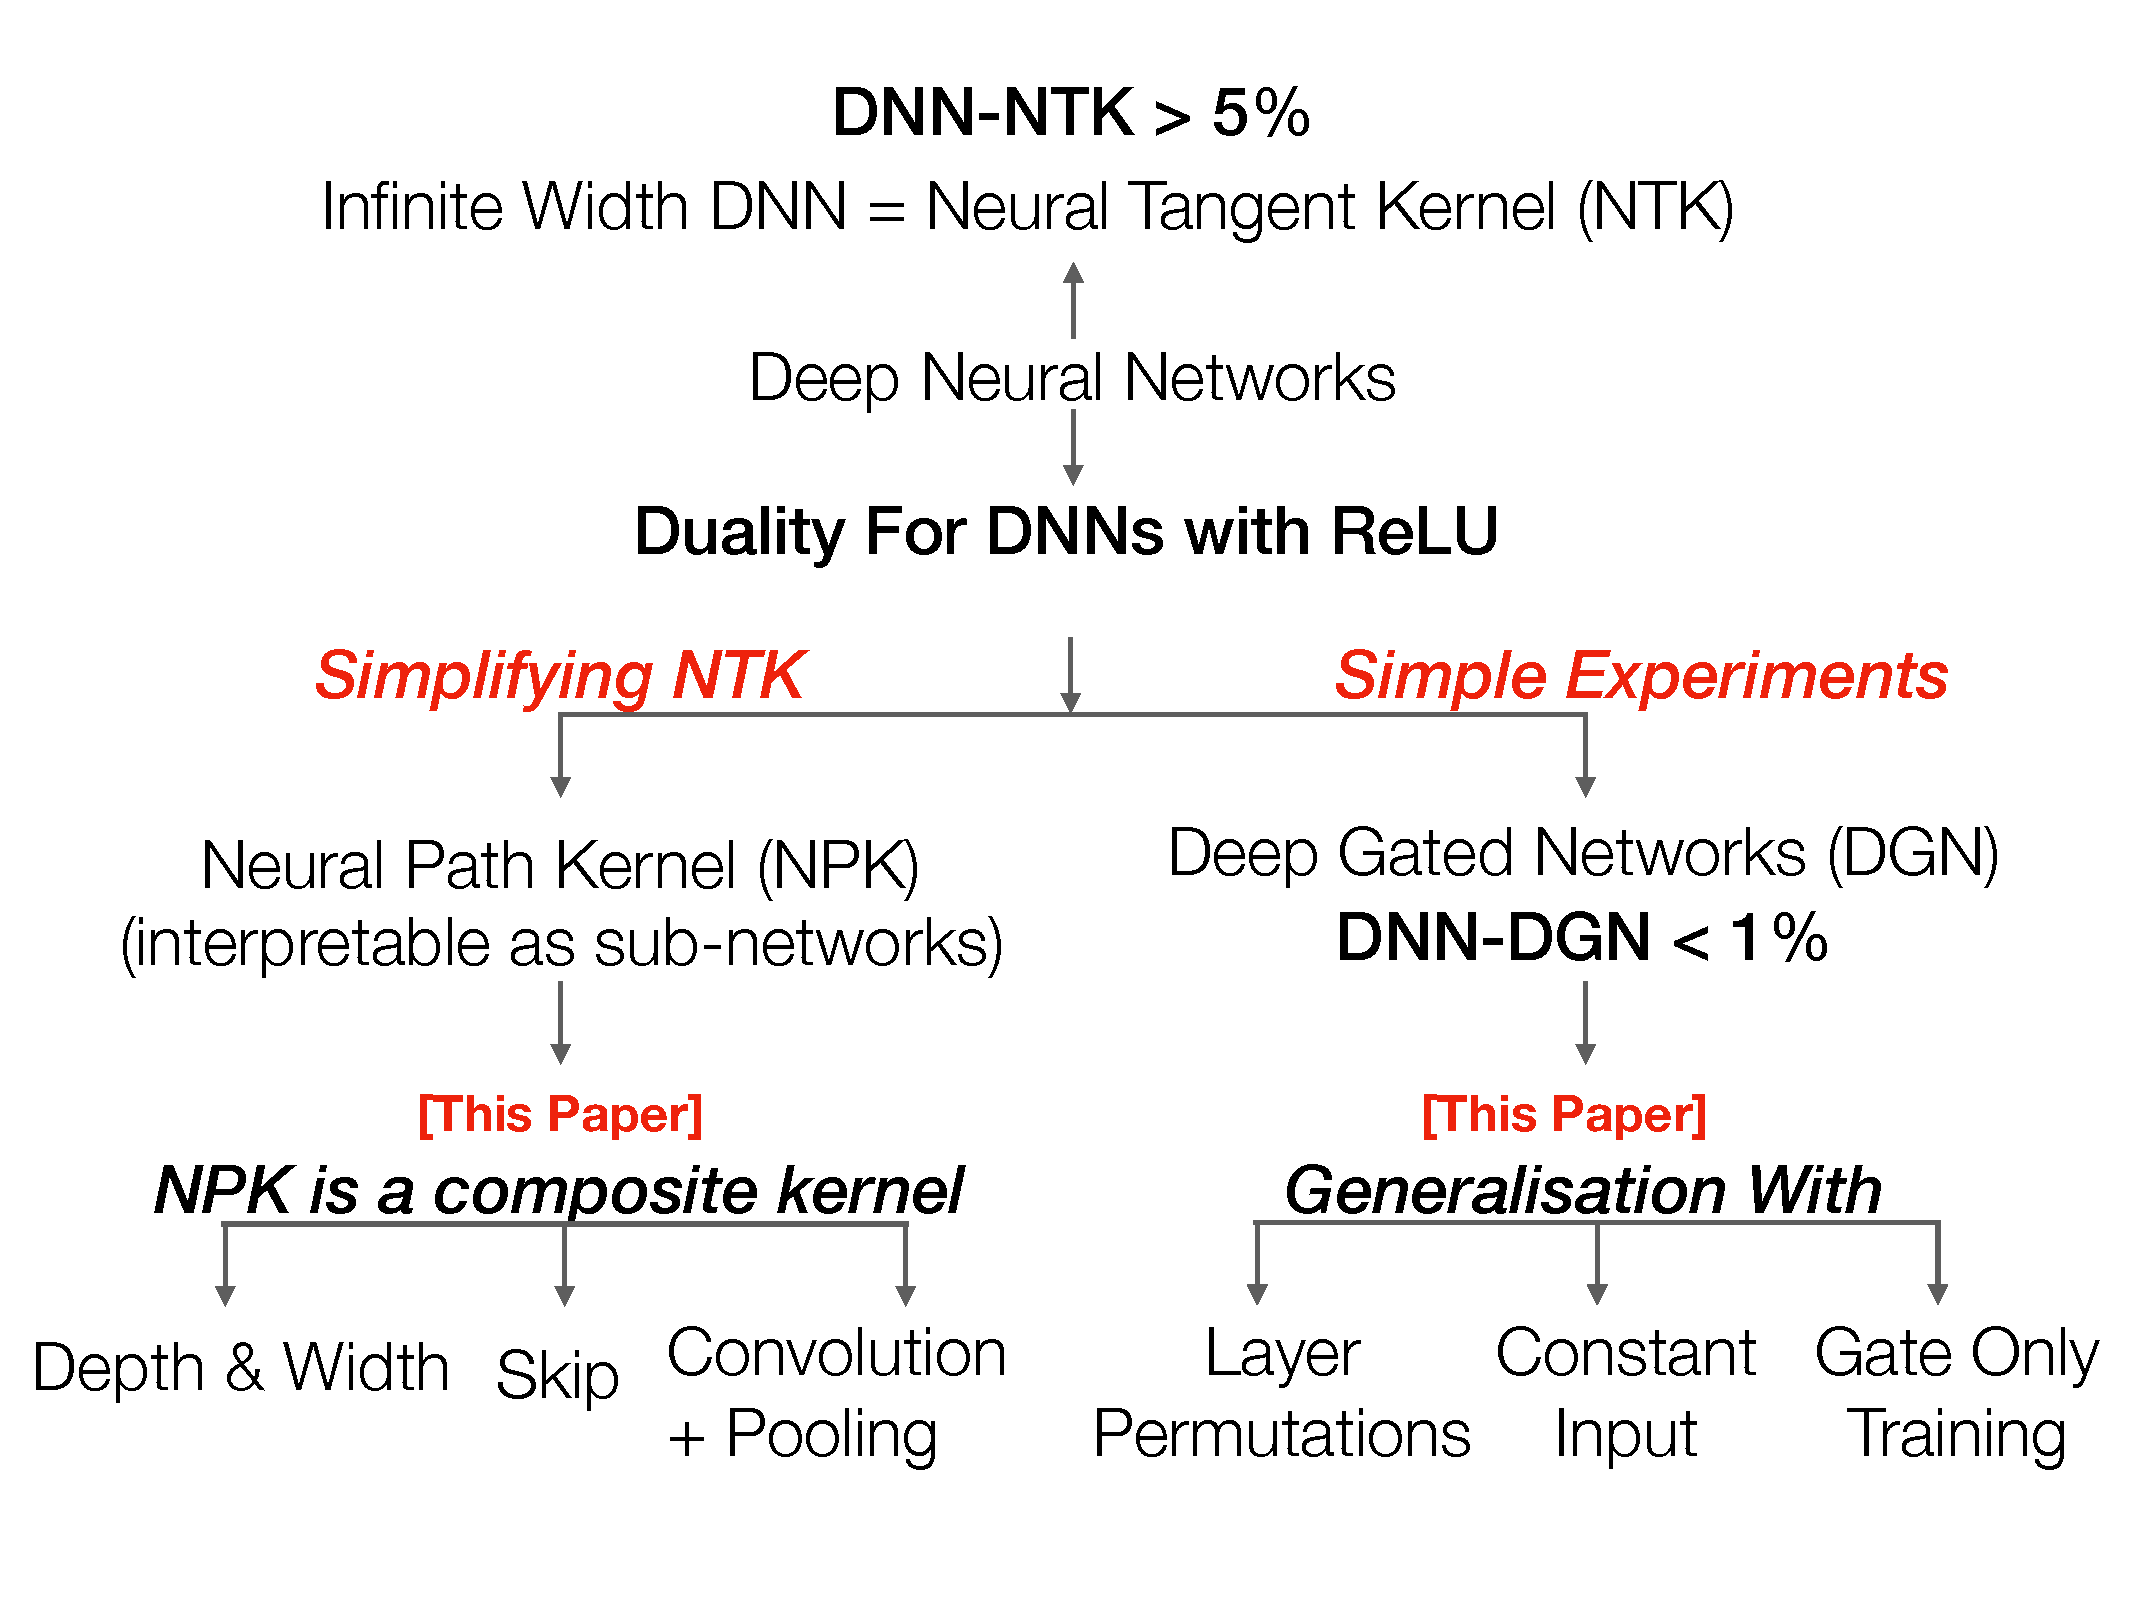
\includegraphics[scale=0.25]{figs/related.pdf}
}
\end{figure}

Table comparing the different kernel methods

\subsection{Our Contributions}

\begin{comment}
 We consider deep neural networks (DNNs) with \emph{rectified linear units} (ReLUs). For such DNNs, we propose a \emph{pedagogical nugget} ``simple theorems, simple experiments" \cite{Aliresponse} by combining \emph{neural tangent kernel} (NTK) and \emph{dual view}. Our aim is to explain training, generalisation, roles of weights/activation/width/depth/convolutions with pooling/skip connections. Training and generalisation of infinite width DNN 


In this paper, we make two major contributions using the lens of dual view. Firstly, we show that the NPK has a \emph{compositional} structure. The results are listed below.

$\bullet$ \emph{Fully Connected DNN (FC-DNN):} In this case, the NPK involves a \emph{ Hadamard product of base kernels} structure. Here the most basic unit is the gate.  stacking ReLUs widthwise in a layer gives rise to a base kernel which measures the \emph{average} number of triggered ReLUs; stacking layers depthwise gives rise to a \emph{Hadamard product}. This result also explains the roles of \emph{width and depth}.

$\bullet$ \emph{Residual networks with skip connections:} In this case, the NPK involves a  \emph{ sum of Hadamard product of base kernels} structure.

$\bullet$ \emph{Convolutional layers with pooling:} In this case, the NPK  has a  \emph{rotational invariant} structure.

Our second major contribution is an ablation study to argue that the standard view that hidden layer outputs is a red-herring and the actual feature learning happens in the gates. To bolster our case, we build combinatorially many models by,

1. permuting the order of the layers when we apply them as external masks,

2. providing a tensor with all entries $1$ instead of the input image. 

We observe in our experiments that the performance is robust to such combinatorial variations.

We also show experimentally how training with random labels affects the gates, and experimentally verify how skip connections improve the conditioning of the underlying NTK.
\end{comment}
\subsection{Organisation}
\subsection{Notation}